\section{实验}
\subsection{实验系统}
为了研究严寒地区新风与回风混合的空气源热泵新风机组的应用特性,在中国哈尔滨建立了如图~\ref{F:1} 所示的实验系统。实验系统主要由室外空气源热泵机组和室内新风处理机组组成。室内机组主要包括室内盘管、混合箱、均流板、调节阀和过滤器等。室外机主要包括变频涡旋压缩机、省煤器、两个电子膨胀阀 (EEV)、气液分离器、油分离器、四通阀、变频风机和翅片盘管。室外机的其他规格参数如表~\ref{T:1} 所示。

压缩机排出的高温高压制冷剂蒸汽进入油分离器,分离出小油滴后,通过四通换向阀进入室内热交换器(热泵机组的冷凝器)。制冷剂在冷凝器中冷却成高温高压的制冷剂液体,然后进入省煤器,分成两股。主回路中的制冷剂经过电子膨胀阀后进入室外热交换器(热泵机组的蒸发器)。吸热汽化后,通过四通换向阀和气液分离器进入压缩机的吸气位置。气液分离器。辅助回路中的制冷剂通过电子膨胀阀节流减压后,在经济器中吸热汽化。辅助回路中的制冷剂通过电子膨胀阀节流减压后,在经济器中吸热汽化,并进入压缩机的喷射位置,形成制冷剂。进入压缩机的喷射位置,形成准二次压缩。

室内实验装置的照片如图所示。进入空气源热泵机组的室内盘管,加热到设定温度后,通过送风口送入室内。然后通过送风管道送入室内。管道送入室内。图~\ref{F:2} 显示了室内机各功能部分的示意图。图~\ref{F:3} 显示了室内机各功能部分的原理图。为了避免室内盘管受热不均,在新风通道后安装了一个略大于新风管道横截面积的均流板、 使新风和回风充分混合。

\begin{figure}[htbp]
	\centering
	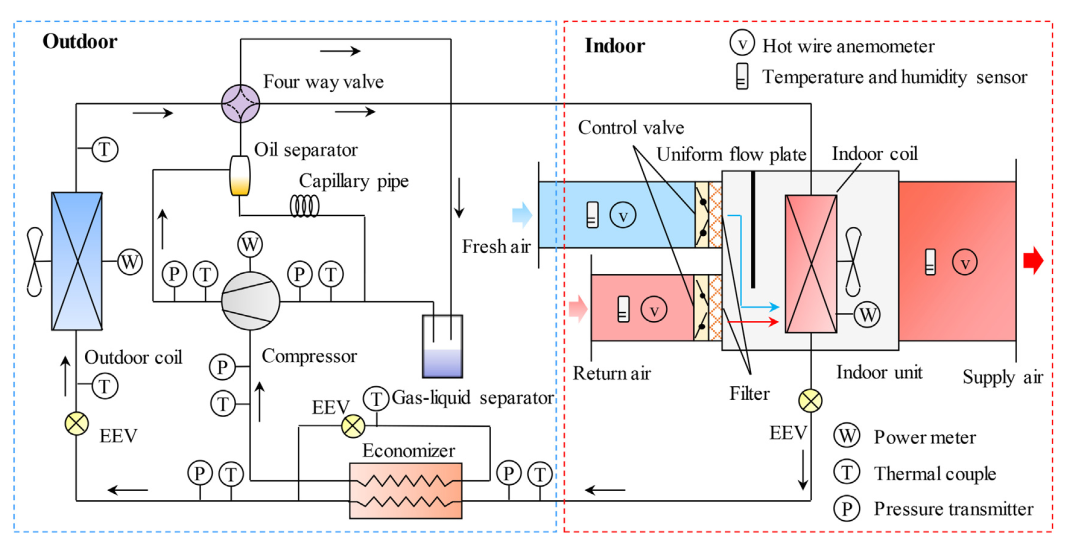
\includegraphics[width=0.7\textwidth]{figure/figure_1}
	\caption{实验系统示意图}
	\label{F:1}
\end{figure}

\begin{table}[ht]
	\centering
	\caption{室外单元参数}
	\begin{tabular}{@{}ll@{}}
		\toprule
		参数 & 值/细节 \\ \midrule
		制冷剂 & R410A \\
		额定制热能力$\unit{\kW} $ & 16.0 \\
		额定输入功率$\unit{\kW} $ & 4.10 \\
		压缩机类型 & 蒸汽喷射涡旋 \\
		压缩机最高转速$\unit{\radian/\s} $ & 120 \\
		外表类型 & 翅片管盘管 \\
		省煤器类型 & Plate \\ \bottomrule
	\end{tabular}
	\label{T:1}
\end{table}

\begin{figure}[htbp]
	\centering
	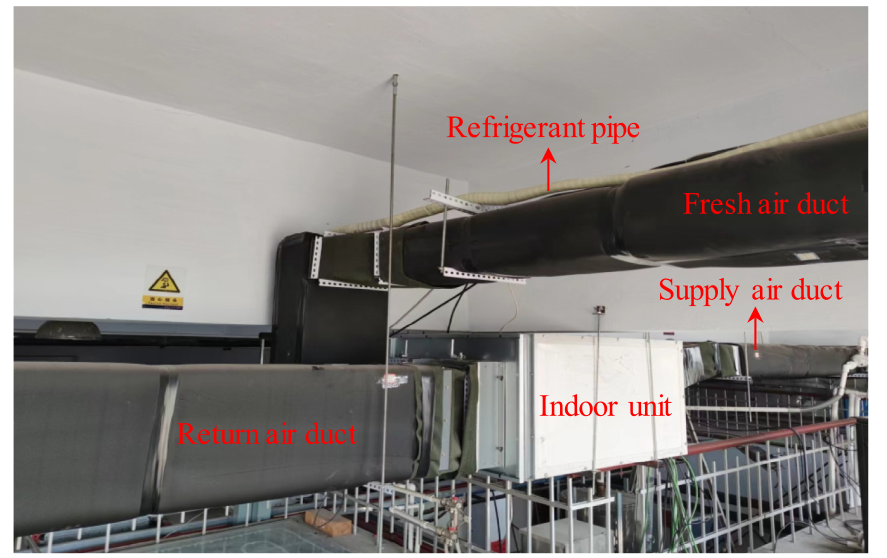
\includegraphics[width=0.7\textwidth]{figure/figure_2}
	\caption{实验设备安装照片}
	\label{F:2}
\end{figure}

\begin{figure}[htbp]
	\centering
	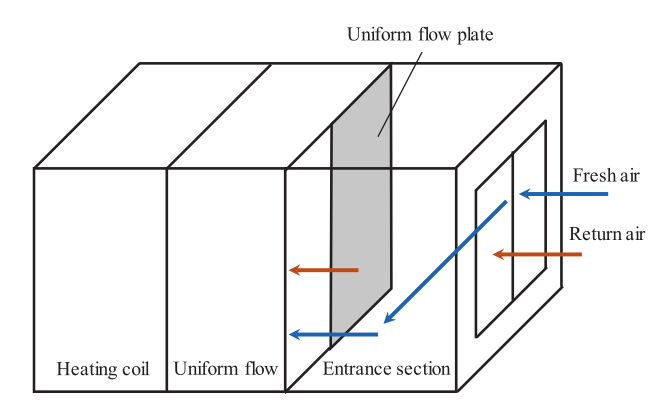
\includegraphics[width=0.7\textwidth]{figure/figure_3}
	\caption{室内机各功能部分示意图}
	\label{F:3}
\end{figure}

\subsection{空气处理过程}
新风装置的设计新风量为$\qty{700}{\m^3/\hour}$。根据标准要求,办公楼内每人所需的最小新风量为$\qty{30}{\m^3/\hour} $。设计新风量可满足至少 23 人的新风需求。此外,新风管道和回风管道都装有过滤器(图~\ref{F:1}),以确保送风质量。此外,实验室还有独立的供暖系统,冬季可将室温保持在$\qty{18}{\degreeCelsius} $。哈尔滨冬季空调室外计算温度为$\qty{27.1}{\degreeCelsius} $,计算相对湿度为 73\%。回风温度和湿度与室内环境一致,为 18\%C/10\%。图~\ref{F:4} 显示了新风机组在特定条件下(新风量为$\qty{700}{\m^3/\hour}$,回风量为 $\qty{1400}{\m^3/\hour} $设定送风温度为$\qty{24}{\degreeCelsius} $的空气处理过程焓湿图。如图~\ref{F:4} 所示,新风状态点 W 和回风状态点 N 混合到 O 点、 此时,混合空气温度为$\qty{3}{\degreeCelsius} $,相对湿度为 19.7\%,从而有效地提高了新风状态下的进风温度。然后将其加热至送风温度状态点 S 湿度比相等。

\subsection{数据采集系统}
为了获取实验数据,实验过程使用了一些仪器。如图~\ref{F:1} 所示,八个制冷剂管道表面安装 T 型热电偶,测量制冷剂温度、五种压力变送器用于测量制冷剂压力,以及两个功率计来测量室内和室外的输入功率。以上所有测试仪器均可输出直流或电压信号并传送至数据采集单元进行存储。数据采集单元以$\qty{6}{\s} $的间隔机率整个实验过程中的所有测试数据。另外,还有四台温湿度记录仪,分别用于记录新风的温湿度、回程、混合空气和送风。

\begin{figure}[htbp]
	\centering
	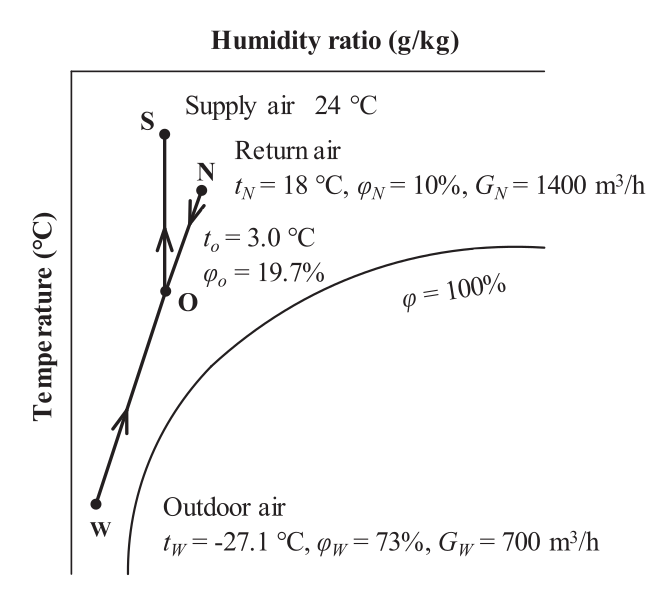
\includegraphics[width=0.5\textwidth]{figure/figure_4}
	\caption{特点条件下的空气处理过程}
	\label{F:4}
\end{figure}

对于测量风量,使用热线风速计用于直接测量空气的平均风速,进而求得风量。标准要求划分矩形风道实验段分成几个面积相同接近正方形的小部分,面积不宜大于$\qty{0.05}{\m^2} $,边长不应大于$\qty{220}{\mm} $,测量点为在每个小部分的中心。图~\ref{F:5} 为各类矩形风道风速测量点示意图。

\begin{figure}[h]
\centering  %图片全局居中
\subfigure[送风管]{
\label{F:5a}
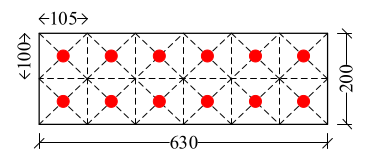
\includegraphics[width=0.3\textwidth]{figure/figure_5_a}}
\subfigure[回风管]{
\label{F:5b}
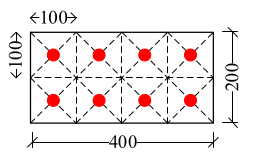
\includegraphics[width=0.3\textwidth]{figure/figure_5_b}}
\subfigure[新风管]{
\label{F:5c}
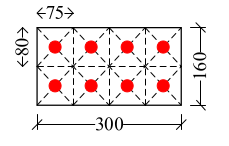
\includegraphics[width=0.3\textwidth]{figure/figure_5_c}}
\caption{风速测点示意图}
\label{F:5}
\end{figure}

各测量仪器的测量精度如表~\ref{T:2} 所示。误差分析见附录。

\subsection{数据处理}
新风和回风的风量由测得风速按公式~\ref{E:1} 计算。
\begin{equation}\label{E:1}
	G = \sum 3600 abv_i
\end{equation}
式中,$G$ 是风道风量,$a, b$小方块长宽,$v_i$为风道内每个测量点的风速。

根据节能原理,供暖新风机组的风量由焓差法根据式~\ref{E:2} 确定。
\begin{equation}\label{E:2}
	Q = \frac{G_W \rho_W (h_S - h_W) + G_N \rho_N (h_S - h_N)}{3600} 
\end{equation}
式中,$Q$是新风机组的制热量,$q, h$分别为空气的密度和热焓,可按下式计算空气的干球温度和相对湿度。这下标$W、N、S$分别代表新风、回风和送风。

新风机组的性能系数 (COP) 按下式~\ref{E:3} 计算:
\begin{equation}\label{E:3}
	COP = \frac{Q}{W} 
\end{equation}
式中,$COP$ 为热泵机组的性能系数,$W$为热泵机组的耗电量,包括压缩机和室外风机的功耗。

压缩机的压缩比按下式~\ref{E:4} 计算:
\begin{equation}\label{E:4}
	r = \frac{P_d}{P_s} 
\end{equation}
式中,$r$外压缩机的压缩比,$P_d$ 和 $P_s$分别为排出压力和吸入压力。

